\subsubsection{Synthesis of ARC with route-filters} \label{sec:routefilter}
\begin{figure}[!t] 
	\centering
	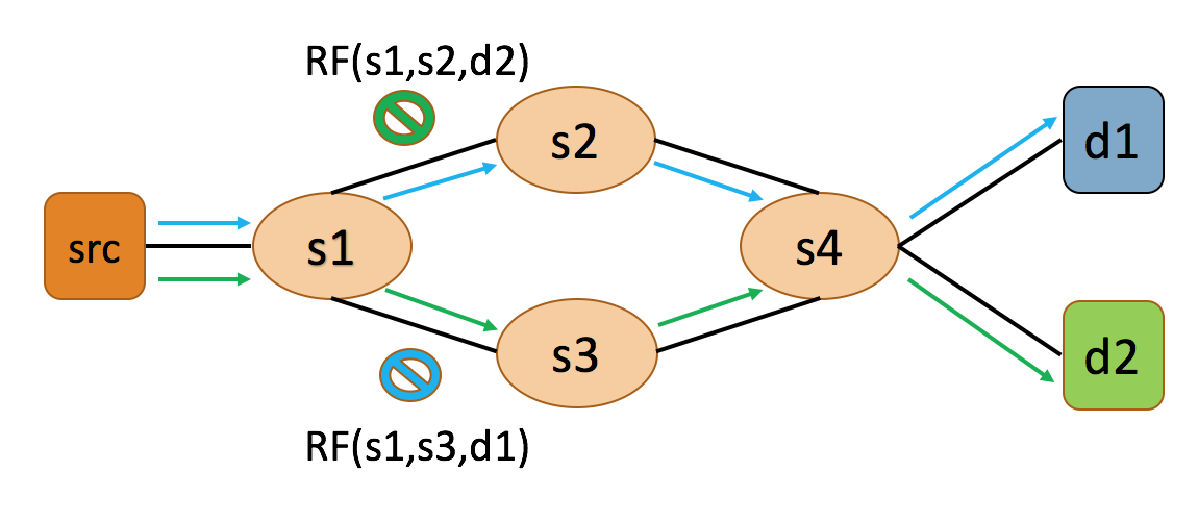
\includegraphics[width=0.7\columnwidth]{figures/diamond.eps}
	\caption{Example of paths that requires route-filtering} \label{fig:diamond}
\end{figure}
The sARC synthesis problem does not always admit a solution.
For example, consider the set of paths illustrated in \Cref{fig:diamond}. 
In this example, both the blue and green paths are required to be the unique shortest paths
and, clearly, this is cannot be enforced for any choice of the edge weights.

In this section, we consider ARCs that use more refined mechanisms to
cope with this problem.
One way to synthesize an ARC in the scenario 
given in \Cref{fig:diamond}
is to ``disable'' the edge
$(s1, s3)$ for destination $d1$.
Using this technique, there is only one possible path from $src$ to $d1$ and the
edge weights become irrelevant for destination $d1$.


This blocking mechanism supported by (non-simplified)
ARC is called a route-filter. 
A route-filter  can selectively disable an
edge for a given destination by  blocking advertisements to a
particular destination along a link. 
Formally, a route-filter is a pair $(l,d)\in L\times S$
disabling a link $l$ for destination $d$
and path to a destination $d$ is \emph{unfiltered} 
if it does not contain edges that are filtered for destination $d$.
%Therefore, if a route-filter is added on switch $s3$, 
%$s3$ 
%will not advertise a route for $d1$ to $s1$, so 
%$s1$ will forward to $s2$ and not to $s3$
%to reach $d1$. The forwarding of packets destined
%for $d2$ are not affected, and they will be sent from
%$s1$ to $s4$ via $s3$ as it is the shortest path.
%Thus, by incorporating route-filters, we can
%disable certain links in the topology 
%for specific destinations, and synthesize
%ARCs for all possible data planes. 
The \emph{ARC synthesis} problem
is to find rational weights for the edges in $L$
and a set of route-filters $F\subseteq L\times S$
 such that 
for each pair of endpoints $(s,t) \in \Gamma$, 
the paths in $P(s,t)$ are the shortest \emph{unfiltered} paths from $s$ to $t$ 
in the graph. 

The ARC synthesis problem admits a trivial solution in which 
route-filters are used to enforce the exact set of input paths by blocking all other possible paths.
This can be done by creating a 
route-filter $(l,d)$ for every link $l$ not in $\xi_d$. 
However, this solution may overly restrict the structure of the network.
In particular, if two nodes were connected by a single path,
a link failure would immediately result in the network becoming disconnected!
Moreover, installing so many route-filters might be costly as not all switches might
support this mechanism.

Ideally, we would like to impose further restrictions to the ARC
synthesis problem to make sure that the obtained solution
satisfy desirable connectivity or resilience properties.
In the following we informally use the word objective 
to identify a property we desire for the synthesized ARC.
Examples of objectives are minimizing the number of route-filters
or maximizing the number of edge-disjoint paths in the ARC
for each endpoint. 
Given an objective $O$, the \emph{augmented ARC synthesis} problem
is to find rational weights for the edges in $L$
and a set of route-filters $F\subseteq L\times S$
 such that 
1) for each pair of endpoints $(s,t) \in \Gamma$, 
the paths in $P(s,t)$ are the shortest \emph{unfiltered} paths from $s$ to $t$ 
in the graph,
2) the resulting ARC satisfies the objective $O$. 
In the following we only allow route-filters for a destination $d$ to be applied to edges of $T$ that are directly connected to 
nodes in $\xi_d$. 

We propose an iterative approach to this problem. 
Our algorithm starts by trying to synthesize a solution
that does not use route-filters using the equations proposed in \secref{sec:sarc}. 
In the case of a failure, the algorithm uses the ``proof of unsatisfiability'' generated by the constraint solver 
to greedily add a small set of route-filters. New equations are then generated and approach is repeated until a solution is found.
We first describe the 
modified linear equations generated when a set of
route-filters are enabled, and then describe two
techniques used to choose route-filters. 
%\begin{figure}
%	\centering
%	\includegraphics[width=\columnwidth]{figures/arcSynthesis.eps}
%	\caption{Synthesis of ARC with route-filters.} \label{fig:arcSynthesis}
%\end{figure}

\minisection{Equations with route-filters}
We show how the technique used to solve the simplified synthesis
problem can be modified to handle filtered and unfiltered paths.
We assume we are given a set of route-filters $F$ and 
use $s\rightarrow_d^* t$ to denote that $s$ can reach $t$
in $T$ without using any edge $l$, such that $(l,d)\in F$.
We use $D_d(sw_1, sw_2)$ to denote the shortest distance from $sw_1$ to $sw_2$
using only edges that are not filtered for destination $d$.
We can revise the equation in \eqref{eq:dist} to correctly restrict the values of $D_d$
by simply ignoring all the filtered edges. 
In the same way, we can modify equations  \eqref{eq:uniq1} and \eqref{eq:uniq2}, while
equation \eqref{eq:uniq3} remains unchanged.

Unfortunately, if the encoding without route-filters produces $n$ equations, this encoding produces $|\Omega|n$ due
to the multiple different distances $D_d$.
Notice that, the shortest distance $D_d(s,t)$ between two nodes $s$ and $t$ without using edges filtered for $d$ cannot be
smaller than the shortest distance $D(s,t)$ obtained without considering route-filters.
We use this property to simplify the encoding by only computing $D(s,t)$ and by replacing each instance of $D_d(s,t)$
with $D(s,t)$ in
equations \eqref{eq:uniq1} and \eqref{eq:uniq2}. 
It is easy to see that every solution of this simplified set of constraints
is also a solution to the original solution (because $D(s,t)\leq D_d(s,t)$).
However, the reverse is not true and the set of simplified equations can be unsatisfiable
in cases in which the original set is satisfiable.
We use the simplified
set of equations in our preliminary implementation and show how it yields encouraging results in practice.

If the set of linear equations does not admit a solution, we 
can add new route-filters so that the equations resulting from the added
route-filters admit a solution.
We discuss two schemes used to add route-filters:
the first scheme uses unsatisfiable cores generated
by the solver and the second scheme 
finds geometrical structures called diamonds that 
cannot be handled without route-filters.


% While detecting diamonds is efficient, the
% presence of diamonds is a not 
% necessary condition for route-filtering.
% Characterising the properties of data planes for which there is
% a pure ARC solution (i.e., no route-filters
% required) is a open algorithmic
% problem. An 
% efficient algorithm to find the structures causing 
% inconsistencies based on these properties 
% can be used to minimize the number of route-filters enabled.  

\minisection{Adding filters using unsatisfiable cores}
Modern LP-solvers have efficient procedures to return an
unsatisfiable core, also called IIS (Irreducible Inconsistent Subsystem)
~\cite{chinneck2007feasibility}. Formally, an IIS is a subset of constraints such that,
if all constraints except those in the IIS are removed, the resulting set of
linear equations is still inconsistent (unsatisfiable). Moreover, the set is irreducible---i.e., removing 
any one constraint of the IIS produces a consistent set of constraints. 

Suppose that, upon producing our set of linear equations, the solver returns unsatisfiable and produces
a concrete unsatisfiable core. 
Some of the linear inequalities from 
Equations \eqref{eq:uniq1} and  \eqref{eq:uniq2}
will appear in the unsat-core 
(an unsat-core cannot consist of only 
constraints from \Cref{eq:dist} and \eqref{eq:uniq3}, as all distances and edges set to zero
would trivially be consistent with these constraints). 
In particular, the unsat-core contains some constraint
\begin{eqnarray}
E(s, n') + D(n', t) > \sum_{\mathclap{\substack{l_i=(s_i,t_i)}}} 
		E(s_i, t_i) 
\end{eqnarray}
that was added to reason about some DAG $\xi_d$.

By adding the route-filter $((s,n'),d)$ to $F$, this inequality is removed from the set of constraints
and the combination of the other constraints appearing in the other unsat-core is now satisfiable.
The complete set of equations may still be inconsistent as other unsat-cores might exist. 
The procedure can be repeated until the resulting set of constraints becomes satisfiable
and we have therefore reached a solution to the ARC synthesis problem.
%\loris{not sure the next paragraph is needed}
%For a given unsat-core, there may be multiple ways to place a route
%filter to eliminate one constraint and we have not investigated
%We can 
%adopt a greedy approach (based on set cover \cite{setcover}) 
%of picking a route-filter which 
%eliminates the maximum number of unsat-cores. However, 
%finding the number of unsat-cores a route-filter eliminates
%is an open problem and instrumental in minimizing the number 
%of route-filters. Other schemes can be used to choose 
%a route-filter from an unsat-core satisfying certain
%objectives. 


\minisection{Diamond elimination}
Finding an IIS is an NP-hard problem~\cite{iiscomplexity}
and can result in slow synthesis times.
We identify a topological property of the set of input paths that 
is guaranteed to require route-filters and use it to produce an initial set of necessary route-filters.
This technique allows us to reduce the number of times we are required to compute  unsat-cores.

We define the structure shown in \Cref{fig:diamond}
as a \emph{diamond}. 
Formally, a problem instance contains a diamond iff there exists two different destinations $d$ and $d'$
such that, in their corresponding DAGs $\xi_d$ and $\xi_{d'}$,
there exists two nodes $s$ and $t$, such that $s\rightarrow_{\xi_d} t$,
$s\rightarrow_{\xi_{d'}} t$, and
there exists a path $l_0\cdots l_n$ from $s$ to $t$ in $\xi_d$ that is not a path from
$s$ to $t$ in $\xi_{d'}$.
As we mentioned at the beginning, synthesizing an ARC for  diamond structures requires
the addition of a route-filter.
In fact, each such a diamond can be ``removed'' by introducing a route-filter $(l_0, d')$ that hides
the path $l_0\cdots l_n$ for the destination $d'$ (see \Cref{fig:diamond}).
Diamonds can detected and removed in polynomial time.
%Consider
%the diamond in \Cref{fig:diamond}. There are two choices
%of route-filters: the $s1-s3$ edge for destination $d1$ 
%and the $s1-s2$ edge for destination $d2$, out of which,
%at least one filter is required to eliminate the 
%inconsistency in the linear equations caused due to the diamond.
%Thus, we find all diamonds for all pairs of destination
%DAGs (this is done in polynomial time) and assign a filter
%to one of the two edges at the source of each diamond. 
%Thus, by removing the diamonds, we can reduce the 
%number of iterations
%of the unsat-core learning approach, which would have 
%provided diamonds as an unsat-core if 
%diamonds were not eliminated.




